\documentclass[12pt]{amsbook}
\usepackage{geometry}                % See geometry.pdf to learn the layout options. There are lots.
%\geometry{letterpaper}                   % ... or a4paper or a5paper or ... 
\geometry{a4paper, top=25mm, right=25mm, bottom=25mm}
%\geometry{landscape}                % Activate for rotated page geometry
\usepackage[parfill]{parskip}    % Activate to begin paragraphs with an empty line rather than an indent
\usepackage{relsize}             % Allows us to define \bigast
\usepackage{graphicx}
\usepackage{amssymb}
\usepackage{epstopdf}
%\usepackage{pause}
\usepackage{wasysym}            
\usepackage{wrapfig}
\DeclareGraphicsRule{.tif}{png}{.png}{`convert #1 `dirname #1`/`basename #1 .tif`.png}

\usepackage{enumerate}
\usepackage{xfrac}

\newcommand{\DD}{\displaystyle}
\newcommand{\R}{\mathbb{R}}

%Tikz
\usepackage{tikz-cd} % For commutative diagrams
\usepackage{tikz-3dplot}
\RequirePackage{pgfplots}
\usetikzlibrary{shadows}
\usetikzlibrary{shapes}
\usetikzlibrary{decorations}
\usetikzlibrary{arrows,decorations.markings} 
\usetikzlibrary{quotes,angles}

\begin{document}
\pagenumbering{gobble}       % This kills the page numbering





\begin{center}
   \textsc{\large MATH 255, Exam 1}\\
\end{center}
\vspace{1cm}

\textbf{Name} \; \underline{\hspace{8cm}}

\vspace{1cm}

\textbf{Instructions} \; No textbook, homework, calculators, phones, or smart watches may be used for this exam. A two-sided 8.5x11" note sheet is acceptable.  The exam is designed to take 50 minutes and must be submitted at the end of the class period. All of your solutions should be easily identifiable and supporting work must be shown. You may use any part of this packet as scratch paper, but please clearly label what work you want to be considered for grading. Ambiguous or illegible answers will not be counted as correct.

\emph{Only the highest scoring \underline{five} problems will be counted towards your total score. You cannot get over 100 points.}

\vspace{1cm}

\textbf{Problem 1} \; \underline{\hspace{1cm}}/20

\vspace{.25cm}

\textbf{Problem 2} \; \underline{\hspace{1cm}}/20

\vspace{.25cm}

\textbf{Problem 3} \; \underline{\hspace{1cm}}/20

\vspace{.25cm}

\textbf{Problem 4} \; \underline{\hspace{1cm}}/20

\vspace{.25cm}

\textbf{Problem 5} \; \underline{\hspace{1cm}}/20

\vspace{.25cm}

\textbf{Problem 6} \; \underline{\hspace{1cm}}/20

\vspace{.5cm}

\textbf{Total} \;\hspace{1.1cm} \underline{\hspace{1.25cm}}/100

\vspace*{4cm}


\begin{center}\large{There are extra pages attached in the back to be used as scratch paper.\\

Feel free to tear these off. If so, write your name on each sheet.}\end{center}










\newpage

\textbf{Problem 1}

\vspace{.25cm}

\begin{enumerate}[(a)]
    \item Draw and clearly label the vectors
\[
\mathbf{v}=\begin{bmatrix} 1 \\ 3 \end{bmatrix} \qquad \mathbf{w}=\begin{bmatrix} 4 \\ 2 \end{bmatrix}
\]
in the plane provided using the provided grid.

\item Evaluate $\mathbf{u}=\mathbf{v}+\mathbf{w}$ and then draw and label $\mathbf{u}$ in the plane.

\item Evaluate $\mathbf{p}=2\mathbf{v}-\sfrac{1}{2}\mathbf{w}$ and then draw and label $\mathbf{p}$ in the plane.

\item Let
\[
\mathbf{A}=\begin{bmatrix} 0 & -1\\ 1 & 0 \end{bmatrix}.
\]
Evaluate
\[
\mathbf{r}=\mathbf{A}\mathbf{v}.
\]
Also, draw and label $\mathbf{r}$ in the plane. 
\end{enumerate}

    \begin{center}
    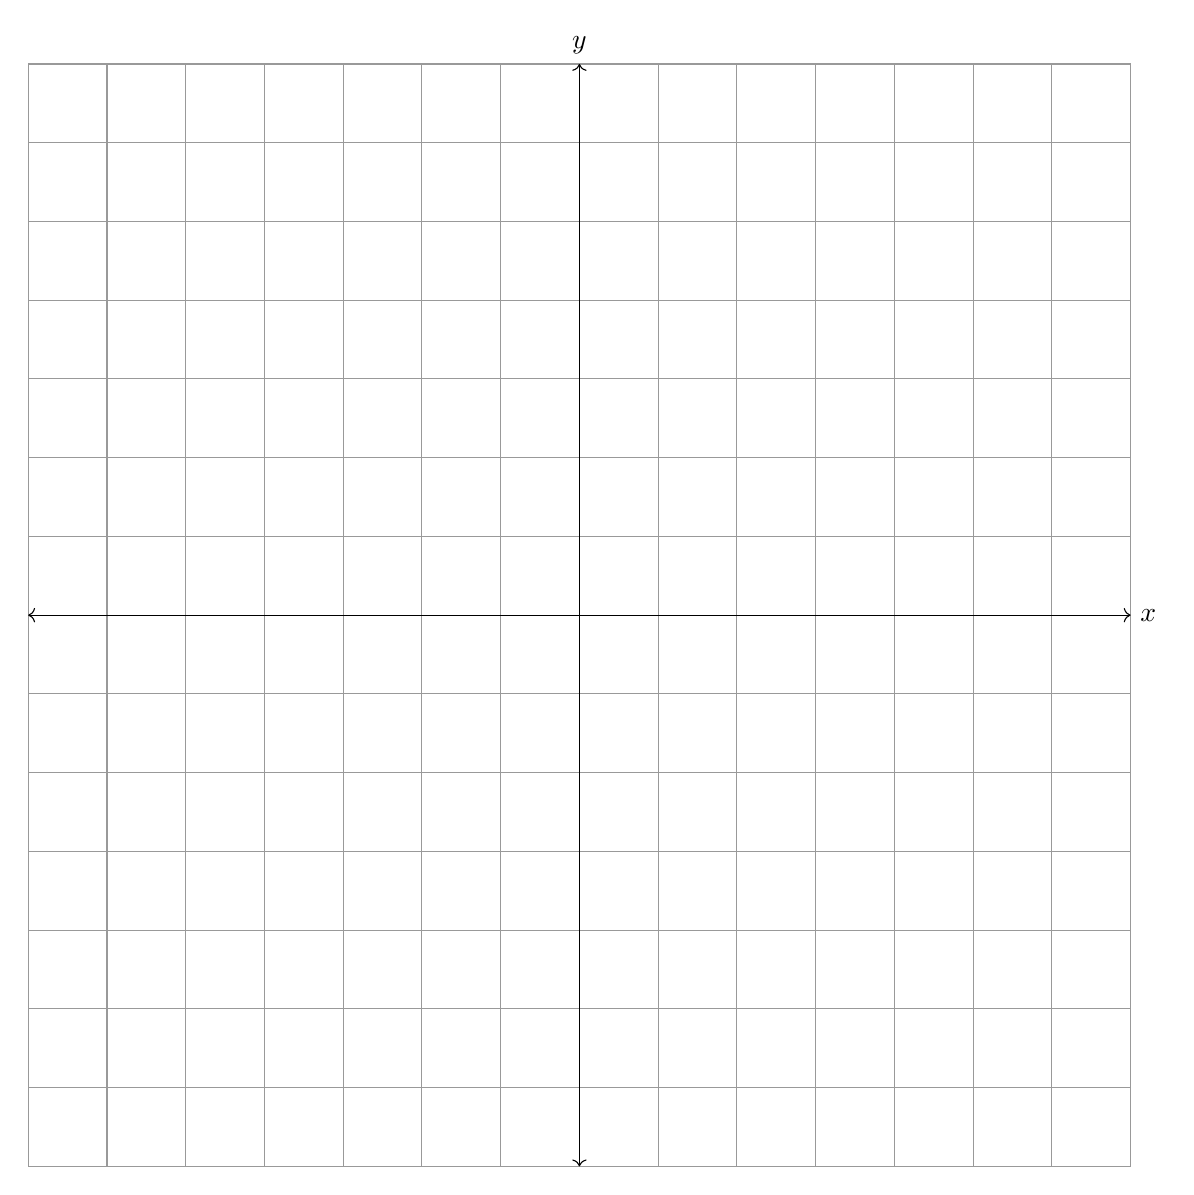
\begin{tikzpicture}
    \draw[thin,gray!80] (-7,-7) grid (7,7);
    \draw[<->] (-7,0)--(7,0) node[right]{$x$};
    \draw[<->] (0,-7)--(0,7) node[above]{$y$};
    \end{tikzpicture}
    \end{center}
    








\newpage

\textbf{Problem 2}

\vspace{.25cm}

\textbf{(i)} \underline{True or false:} Let $\mathbf{a}$ and $\mathbf{b}$ both be vectors in $\R^3$ (3-dimensional space). Then $\mathbf{c}=\mathbf{a}\times \mathbf{b}$ is always orthogonal to both $\mathbf{a}$ and $\mathbf{b}$.
\vspace*{2cm}

\noindent\textbf{(ii)} Let
\[
\mathbf{a}=\begin{bmatrix} 1 \\ 1\\ 1\\ \end{bmatrix} \qquad \mathbf{b}=\begin{bmatrix} 3 \\ 0 \\ 3\\ \end{bmatrix}.
\]
\begin{enumerate}[(a)]
    \item Compute $\mathbf{c}=\mathbf{a}\times \mathbf{b}$.
    \item Compute $\|\mathbf{c}\|$.
    \item What is the angle $\theta$ between $\mathbf{a}$ and $\mathbf{b}$? Do not worry about simplifying your answer!
\end{enumerate}

\vspace*{6cm}

\textbf{(iii)} Let
\[
\mathbf{F}=\begin{bmatrix} 5 \\ 10 \\ 0 \end{bmatrix} \qquad \mathbf{r}= \begin{bmatrix} -2 \\ c\\ 4 \end{bmatrix}.
\]

The \emph{work} $W$ done by the force $\mathbf{F}$ on the object displaced by $\mathbf{r}$ is
\[
W=\mathbf{F}\cdot \mathbf{r}.
\]
For what value of $c$ is zero work done?





\newpage

\textbf{Problem 3}

\vspace{.25cm}

\textbf{(i)} \underline{True or false:} The following transformations are linear. \\

\begin{enumerate}[(a)]
    \item 
    $\DD{T_a(x)=5x+1}$. 
    \item $\DD{T_b\left(\begin{bmatrix} x\\ y \end{bmatrix} \right) = \begin{bmatrix} x+2y\\ 2x + y \end{bmatrix}}.$
    \item $\DD{T_c\left( \begin{bmatrix} x\\ y\\ z\\ \end{bmatrix} \right) = \begin{bmatrix} 0 \end{bmatrix}}$.
\end{enumerate}
\vspace*{1cm}

\noindent \textbf{(ii)} Find the matrix $\mathbf{A}$ so that for 
\[
\mathbf{v}=\begin{bmatrix}
x\\ y \\ z
\end{bmatrix}
\]
we have
\[
\mathbf{Av}=\begin{bmatrix} 0\\ 1x+1z\\ 2z\end{bmatrix}.
\]

\vspace*{8cm}

\noindent \textbf{(iii)} \underline{True or false:} Every linear transformation $T$ of a vector $\mathbf{v}$ can be written as a matrix times the vector $\mathbf{v}$.

\underline{If false, explain why.}








\newpage

\textbf{Problem 4}

\vspace{.25cm}

\noindent\textbf{(i)} Let
\[
\mathbf{M}= \begin{bmatrix} 1 & 2\\ 0 & 1 \end{bmatrix} \qquad \mathbf{N}=\begin{bmatrix} 5 & 0\\ 5 & 5 \end{bmatrix} \qquad \mathbf{P}=\begin{bmatrix} 1 & 0 & 1\\ 2 & 0 & 2 \end{bmatrix}.
\]
For the following, determine whether the matrix expression is possible to compute.  If so, compute it.
\begin{enumerate}[(a)]
    \item $\mathbf{NM}-\mathbf{MN}$.
    \item $\mathbf{PM}$.
    \item $\mathbf{MP}$.
\end{enumerate}

\vspace*{10cm}

\noindent\textbf{(ii)} Let 
\[
\mathbf{A}= \begin{bmatrix} 5 & 3 & 3 \\ 0 & 4 & 1\\ 0 & 1 & 2 \end{bmatrix}.
\]
Compute $\det(\mathbf{A})$.


\vspace*{4cm}

\newpage
\textbf{Problem 4, continued.}

\noindent\textbf{(iii)} Let 
\[
\mathbf{v}=\begin{bmatrix} 1\\ 2 \end{bmatrix} \qquad \mathbf{w}=\begin{bmatrix} 4 \\ 2 \end{bmatrix} \qquad \mathbf{A}= \begin{bmatrix} \mathbf{v} & \mathbf{w}\end{bmatrix}= \begin{bmatrix} 1 & 4\\ 2 & 2\end{bmatrix}.
\]

Geometrically, what does $|\det(\mathbf{A})|$ represent? Draw and label this in the plane below.
    \begin{center}
    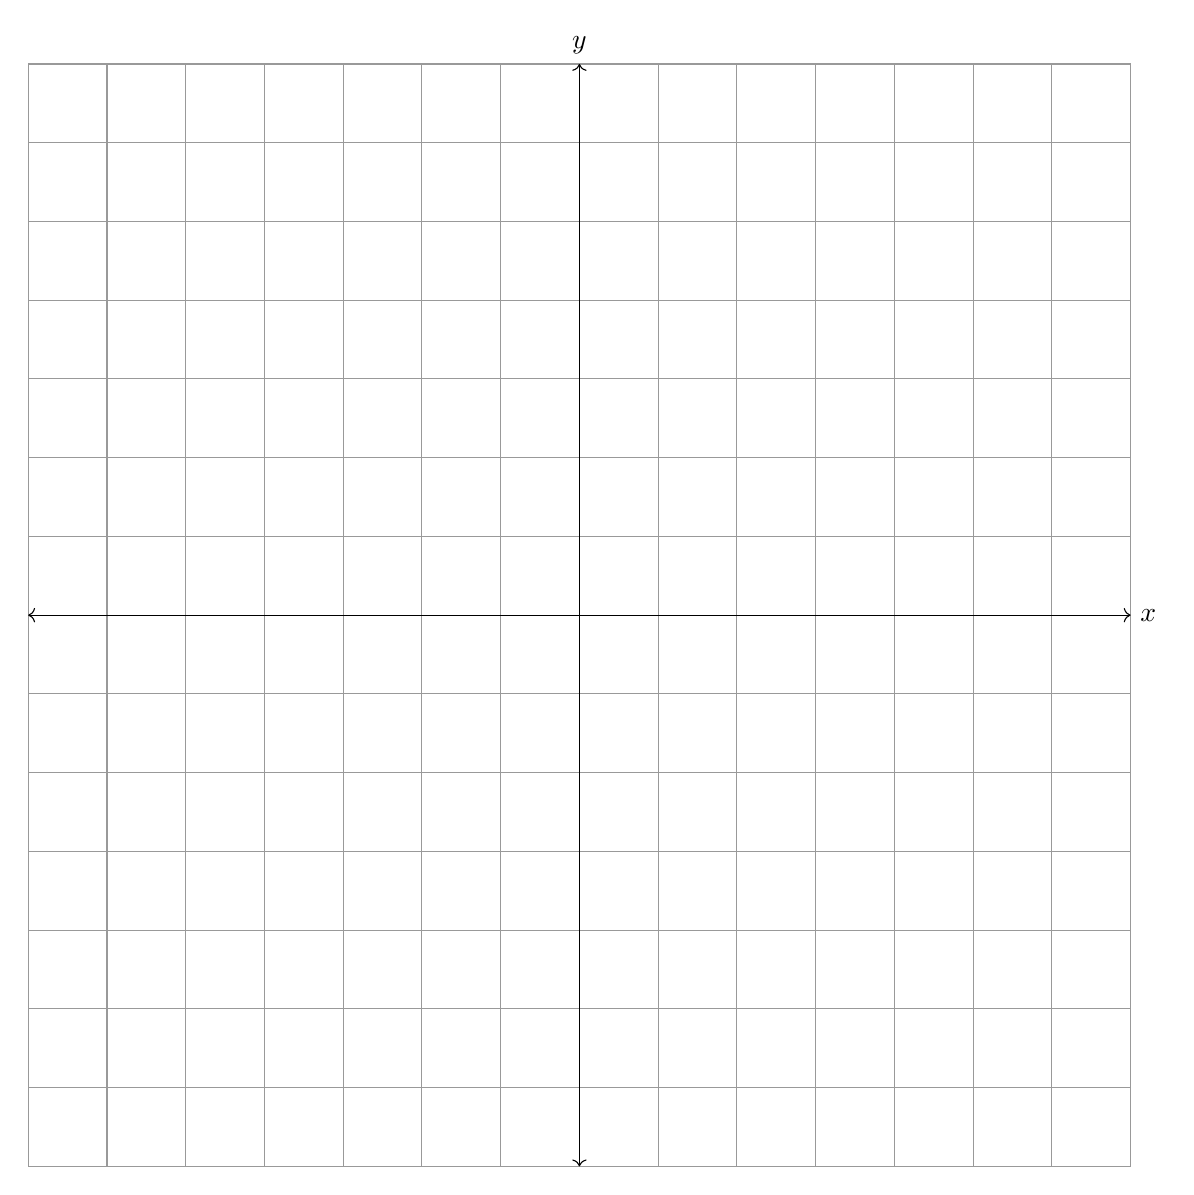
\begin{tikzpicture}
    \draw[thin,gray!80] (-7,-7) grid (7,7);
    \draw[<->] (-7,0)--(7,0) node[right]{$x$};
    \draw[<->] (0,-7)--(0,7) node[above]{$y$};
    \end{tikzpicture}
    \end{center}












\newpage

\textbf{Problem 5}

\vspace{.25cm}

\noindent\textbf{(i)} Consider the following system of equations
\begin{align*}
    1x+2y+0z&=3\\
    -1x-1y-1z&=-6\\
    1x+2y+1z&=8.
\end{align*}
Find a solution to the system of equations. (\emph{For less points, just explain how you would find the solution.})

\vspace*{10cm}

\noindent\textbf{(ii)} Given
\[
\mathbf{A}=\begin{bmatrix} 1 & 1 \\ \sfrac{1}{2} & 0 \end{bmatrix}.
\]
Find $A^{-1}$.  Show that the inverse matrix you found is correct.













\newpage

\textbf{Problem 6} 

\vspace{.25cm}

Let
\[
\mathbf{A}=\begin{bmatrix} -3 & 5\\ 0 & 2\end{bmatrix}.
\]
\begin{enumerate}[(a)]
    \item Find the eigenvalues of $\mathbf{A}$.
    \item Find the corresponding eigenvectors.
    \item Show that the eigenvalues and eigenvectors you found are correct.  That is, verify they satisfy the eigen-equation
    \[
    \mathbf{A}\mathbf{v}=\lambda \mathbf{v}.
    \]
\end{enumerate}



\newpage
\emph{Intentionally left blank to be used as scratch paper.}\\

\textbf{Name:} \underline{\hspace*{8cm}}

\newpage
\emph{Intentionally left blank to be used as scratch paper.}\\

\textbf{Name:} \underline{\hspace*{8cm}}









\end{document}  